\documentclass[11pt,a4paper]{article}
\usepackage[utf8]{inputenc}
\usepackage[T1]{fontenc}
\usepackage{lmodern}
\usepackage[french]{babel}
\usepackage[margin=2.1cm]{geometry}
\usepackage{microtype}
\usepackage{amsmath,amssymb}
\usepackage{booktabs}
\usepackage{array}
\usepackage[table]{xcolor}
\usepackage{graphicx}
\usepackage{caption}
\usepackage{eurosym}
\usepackage[most]{tcolorbox}
\definecolor{navy}{HTML}{1F3864}
\definecolor{bluemid}{HTML}{2E5496}
\definecolor{lightblue}{HTML}{D6E0F0}
\captionsetup{font=small,labelfont={bf,color=navy},labelsep=period}
\graphicspath{{../figures/}}
\newtcolorbox{cle}[1][]{colback=lightblue!40,colframe=navy,boxrule=0.6pt,
  arc=2pt,left=8pt,right=8pt,top=6pt,bottom=6pt,#1}

\title{\vspace{-1.2cm}\color{navy}\bfseries Le SCR, quantile d'un objet incertain\\[2pt]
  \large VaR prédictive et VaR robuste, deux réponses}
\author{Kélian Kaddouri}
\date{27 juillet 2026}

\begin{document}
\maketitle
\vspace{-0.9cm}

\begin{cle}
\textbf{La remarque de Caroline Hillairet.} Estimer le SCR par un \textbf{quantile} (VaR
$99{,}5\,\%$) est fragile car les données elles-mêmes sont incertaines : \og{}le quantile d'un
objet incertain est mauvais\fg{}. On ne peut pas abandonner la VaR (elle est imposée par le cadre
prudentiel), mais on peut traiter son estimation honnêtement, de deux manières complémentaires.
\end{cle}

\medskip
\noindent\textbf{La VaR prédictive} intègre l'incertitude de paramètre \emph{avant} de prendre le
quantile : on prend le quantile de la loi \emph{prédictive}, mélange des GPD sur la distribution
bootstrap de $(\xi,\sigma)$. Résultat instructif : à $99{,}5\,\%$ elle est \emph{quasi égale} au
\emph{plug-in} ($657$ contre $659$~M\euro). Le risque d'estimation n'est pas un biais de
\emph{point} à ce niveau ; il ne le devient qu'en profondeur ($+6\,\%$ à $99{,}9\,\%$). La
fragilité est dans la \textbf{largeur} de la bande (facteur $2{,}6$ sur la VaR, bien plus sur la
TVaR), pas dans le point.

\begin{center}
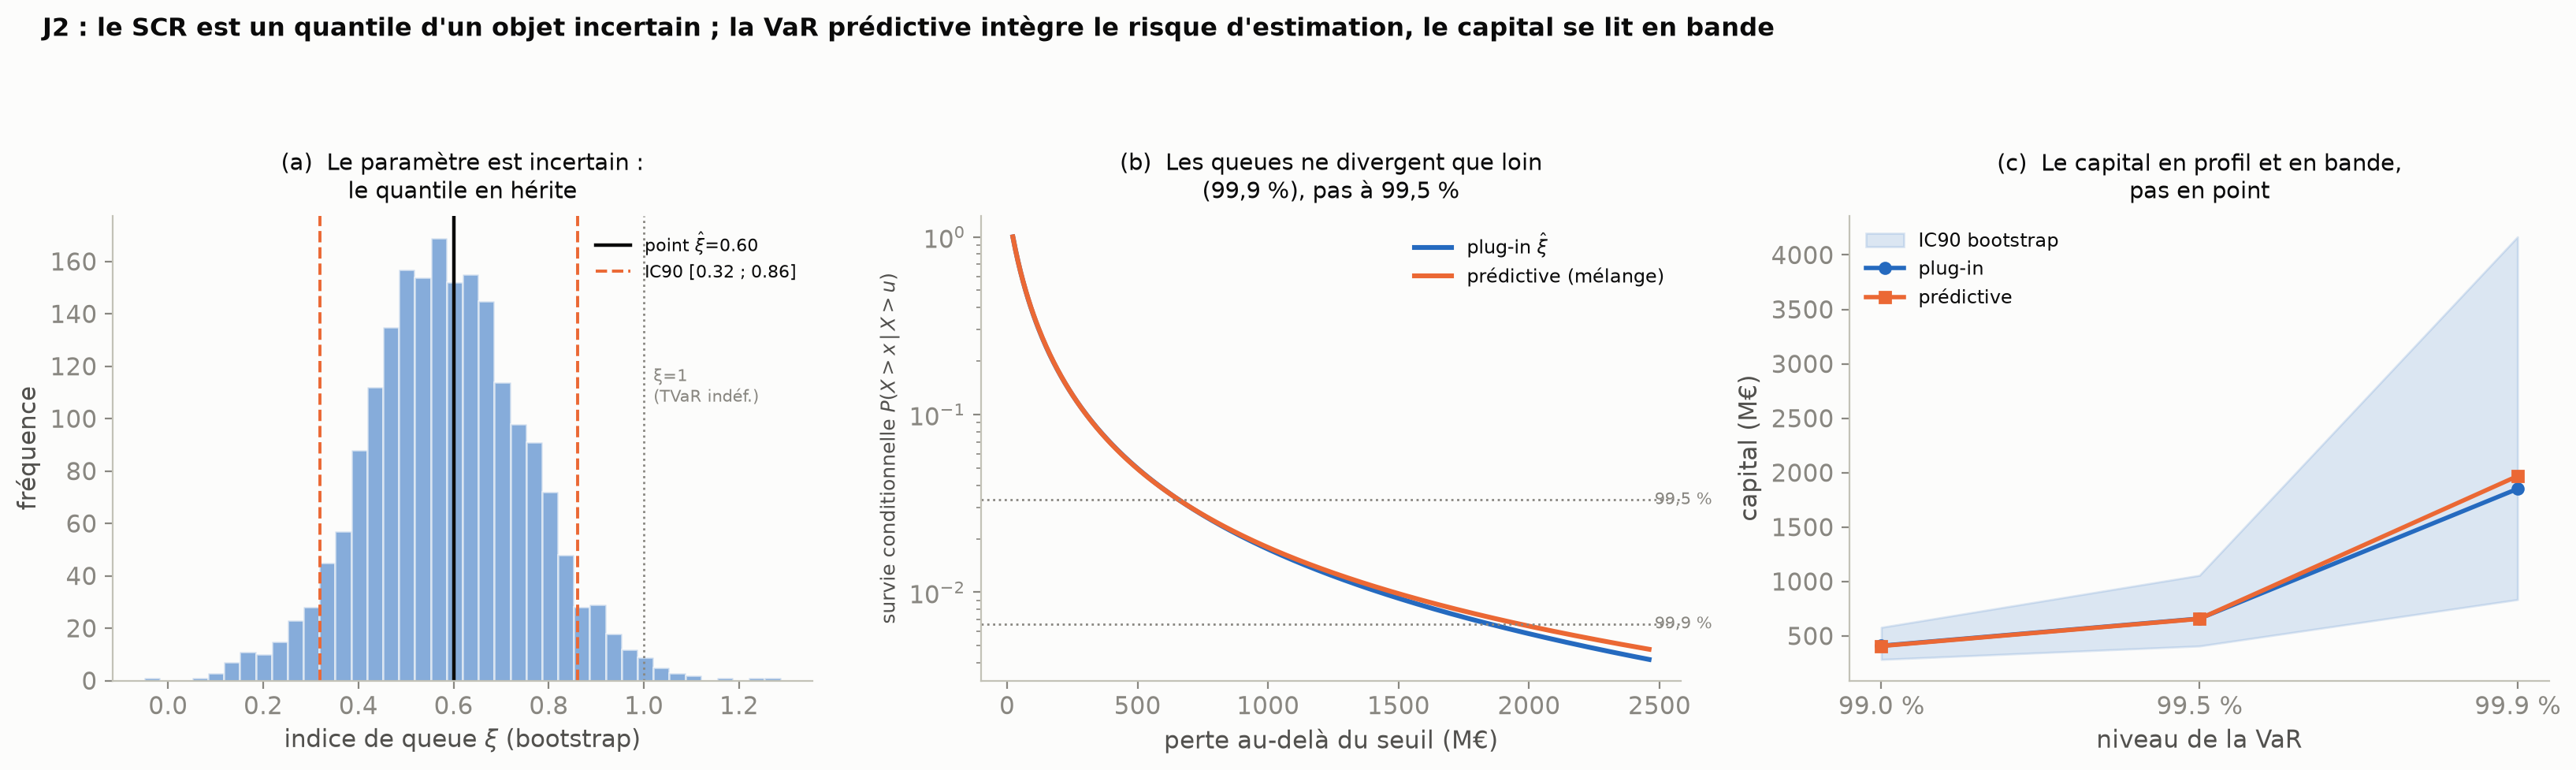
\includegraphics[width=\linewidth]{J2_var_predictive.png}
\captionof{figure}{VaR prédictive. \textbf{(a)} le paramètre $\xi$ est incertain. \textbf{(b)} les
queues \emph{plug-in} et prédictive ne divergent que loin dans la queue. \textbf{(c)} le capital
se lit en profil et en bande.}
\end{center}

\noindent\textbf{La VaR robuste} prend au contraire la \textbf{borne haute} de la VaR sur
l'ensemble d'ambiguïté (paramètre, puis modèle). La VaR robuste à $95\,\%$ vaut $1\,026$~M\euro{}
($1{,}6\times$ le \emph{plug-in} $659$) ; le pire-cas de famille lourde, $1\,311$~M\euro. Le
niveau de robustesse est un \textbf{choix prudentiel explicite}.

\begin{center}
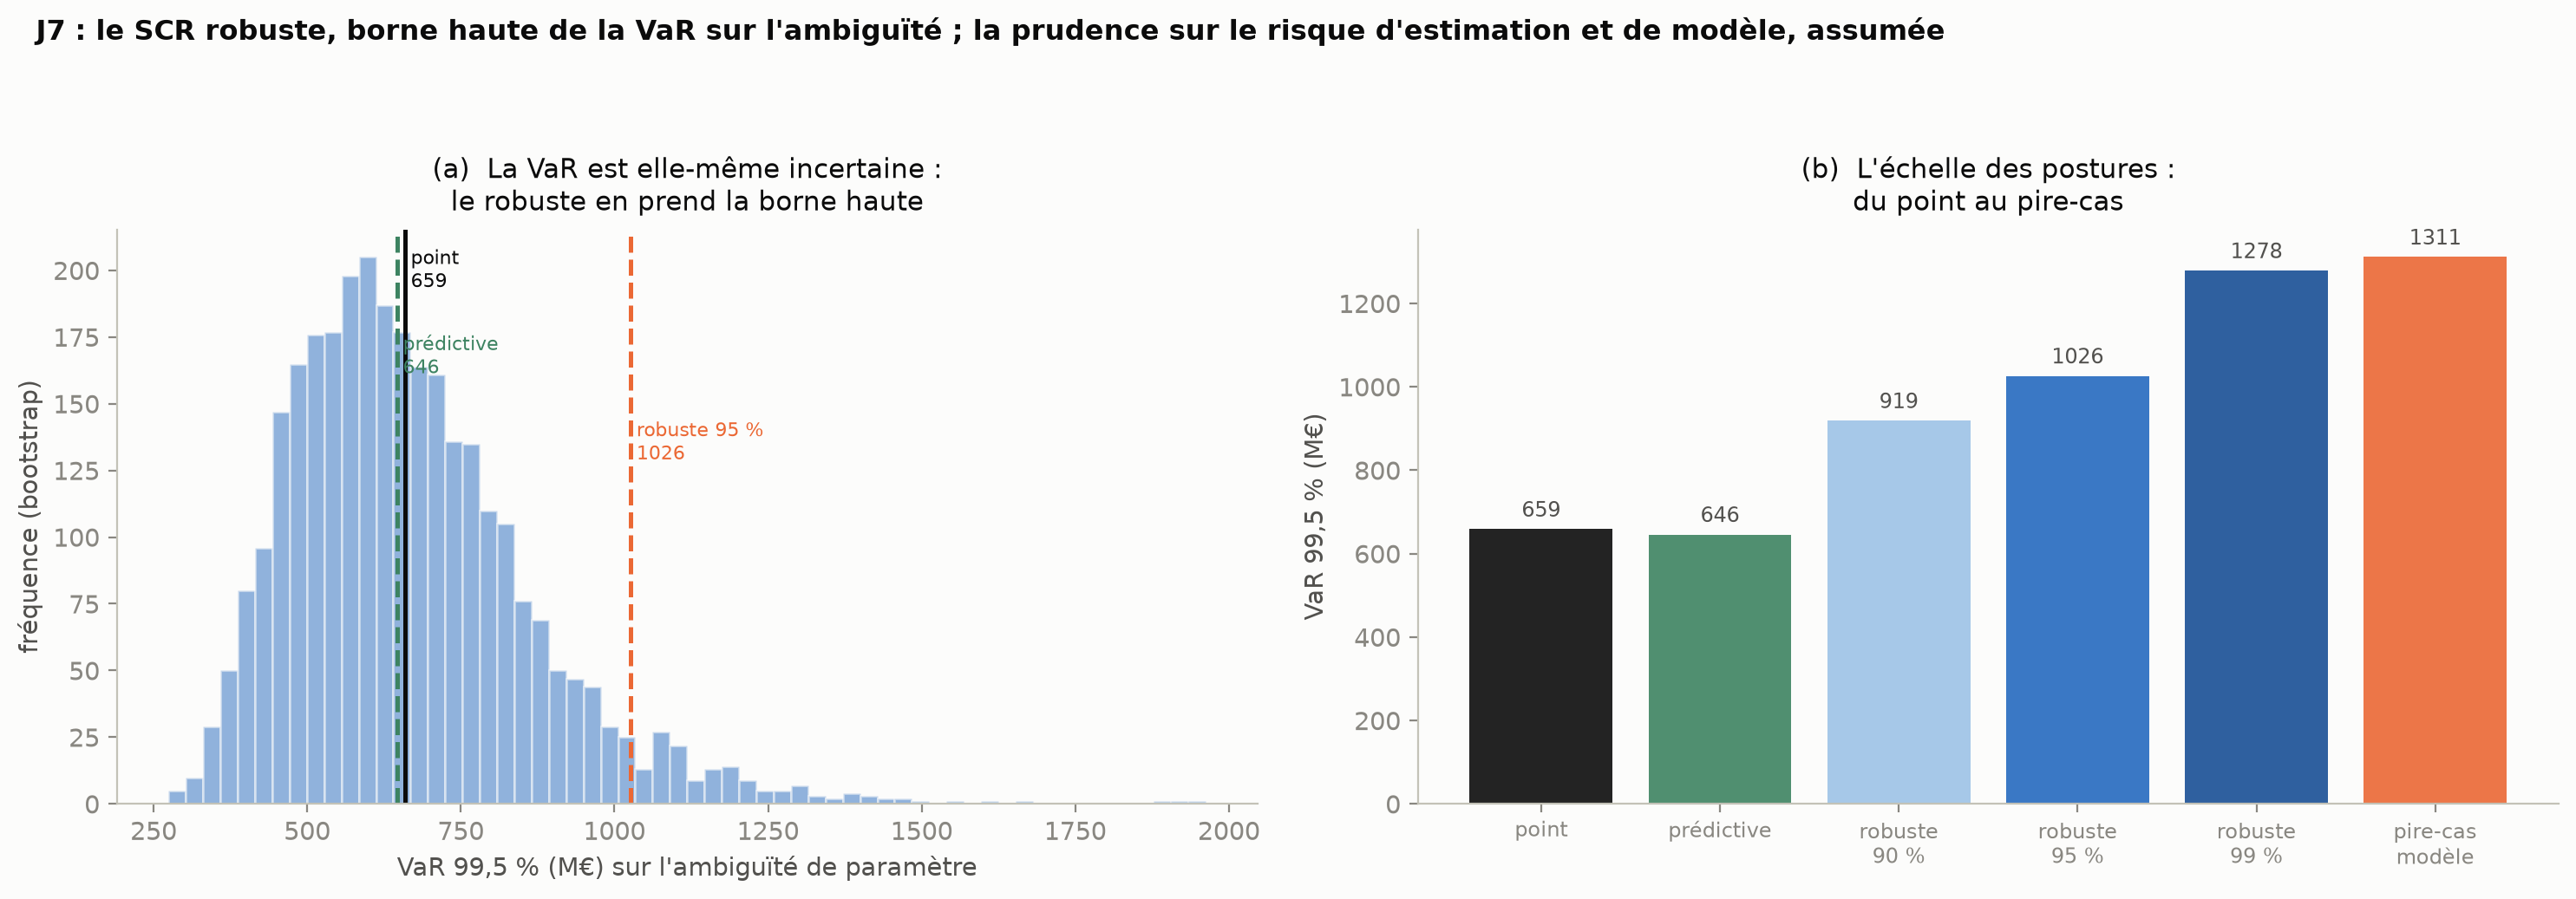
\includegraphics[width=\linewidth]{J7_scr_robuste.png}
\captionof{figure}{VaR robuste. \textbf{(a)} la VaR est elle-même incertaine ; le robuste en prend
la borne haute. \textbf{(b)} l'échelle des postures, du point ($659$) au pire-cas de modèle
($1\,311$~M\euro).}
\end{center}

\begin{cle}
\textbf{Deux points honnêtes plutôt qu'un point trompeur.} La VaR prédictive est le point
\emph{honnête} (il embarque l'incertitude d'estimation) ; la VaR robuste est le point
\emph{prudent} (la borne haute sur l'ambiguïté). Le choix relève de la politique prudentielle,
non du calcul. L'essentiel est de ne jamais reporter le seul \emph{plug-in} : le SCR se cite avec
sa bande, ou par un point qui assume l'incertitude, jamais nu.
\end{cle}

\smallskip
\noindent\footnotesize\textcolor{navy}{\textbf{Source.}} Scripts
\texttt{1\_fondations/46\_var\_predictive.py} et \texttt{51\_scr\_robuste.py}, figures
\texttt{J2} et \texttt{J7}. Calibration OpRisk, bootstrap paramétrique.

\end{document}
